\subsection{Finite Elemente und Formfunktionen}
\label{sec:finite_elements_and_shape_functions}
Ein häufiger Ansatz zur Unterteilung des Problemgebietes ist jener der Unterteilung in Dreiecke bzw. Tetraeder. Innerhalb jedes dieser Elemente wird die gesuchte Funktion $u$ aus \ref{eq:operatorgleichung}, im Weiteren auch Potential genannt, durch einfache Funktionen, meist Polynome erster oder zweiter Ordnung, angenähert.\newline
Für ein Element, welches durch $N$ Knoten definiert wird lautet ein möglicher Ansatz 
\begin{equation}
\label{eq:ansatz_potential}
u(x,y) = \sum_{k = 1}^{N_e}N_k^e u_k
\end{equation}
wobei die Funktionen $N_k^e$ als \textit{Formfunktionen} des $e$-ten Elements bezeichnet werden. Sie besitzen im $k$-ten Elementknotenknoten den Wert $1$ und in allen Anderen den Wert $0$. \newline
Für ein Dreieck mit einem Knoten an jeder Ecke ($N = 3$) ergeben sich lineare Funktionen für $N_k^e$, für Dreiecke mit zusätzlichen Knoten in der Mitte jeder Seite ($N=6$) quadratische Funktionen usw. \newline
Da die Funktionen für $N_k^e$ nur von der Geometrie des jeweiligen Elements abhängen bleiben einzig die $u_k$ als gesuchte Parameter, welche durch Verwendung des Ansatzes aus ($\ref{eq:ansatz_potential}$) im z.B. Galerkinschen Verfahren ermittelt werden können.\newline

Wie aus ($\ref{eq:ansatz_potential}$) erkennbar, müssen für jedes Element die $N_k^e$ separat ermittelt werden da sie von der jeweiligen Elementgeometrie abhängen. Betrachtet man nun jedes finite Element in einem lokalen Koordinatensystem, welches im Weiteren durch die Variablen $\xi,\eta$ dargestellt wird, und verwendet die Formfunktionen auch zur Beschreibung der Elementgeometrie, so spricht man von \textit{isoparametrischen finiten Elementen.}\newline
Die Formfunktionen müssen dabei nur einmalig für einen bestimmten Typ von finten Elementen (z.B. lineare Dreicke) einmalig ermittelt werden. Die Zusammenhänge für Geometrie und Potential lauten dann wie folgt:
\begin{equation}
\label{ref:ansatz_isoparam}
u = \sum_{k = 1}^{N} N_k(\xi, \eta) u_k \quad x = \sum_{k = 1}^{N} N_k(\xi, \eta) x_k  \quad y = \sum_{k = 1}^{N} N_k(\xi, \eta) y_k \nonumber
\end{equation}
wobei $x_k$ und $y_k$ die Koordinaten des $k$-ten Knoten darstellen. Sinnvollerweise sind die jeweiligen finiten Elemente im lokalen $\xi,\eta$-Koordinatensystem geradlinig angesetzt. (Siehe Abbildung \ref{fig:quadratic_element} ) Die Krümmung und Verzerrung im globalen Koordinatensystem ergibt sich anschließend durch (\ref{ref:ansatz_isoparam}).



\subsubsection{Lineare Dreieckselemente}
\label{sec:linear_triangles}
Das isoparametrische lineare Finite Dreieckselement ist im lokalen $\xi,\eta$-Koordinatensystem wie in Abbildung \ref{fig:linear_element} gezeigt dargestellt. \newline

\begin{wrapfigure}{r}{8cm}
	\begin{center}
		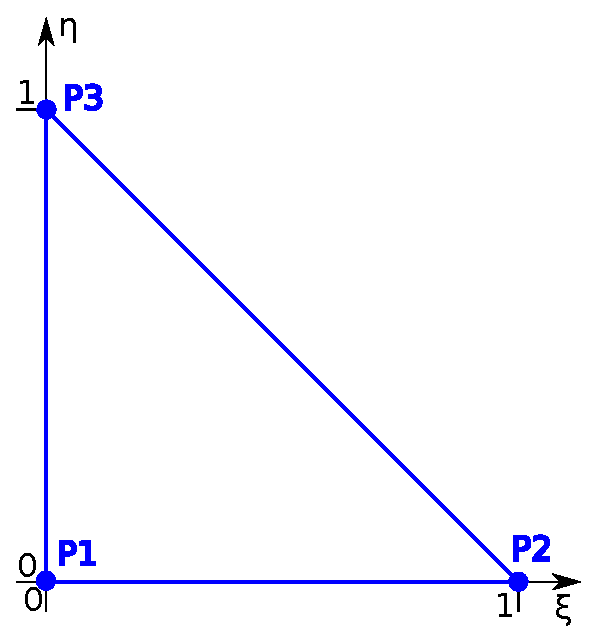
\includegraphics[scale=0.65]{pics/linear_element.eps}
	\end{center}
	\caption{Ansatz für lineares Element}
	\label{fig:linear_element}
\end{wrapfigure}

Die Koordinaten der drei Elementknoten lauten wie folgt:
\begin{align}
&P_1 = \coord{0}{0}, \quad P_2 = \coord{0}{1} \\
&P_3 = \coord{1}{0} \nonumber
\end{align}

Als Ansatz für die Potentialfunktion bzw. die globalen Koordinaten $x$ und $y$ wählt man folgenden Ansatz:
\begin{equation}
 \label{eq:linear_triangle_eq}
u(\xi, \eta) = c_0 + c_1 \xi + c_2 \eta
\end{equation}
Die drei Unbekannten $c_0$, $c_1$ und $c_2$ können durch Einsetzen der Koordinaten der Elementknoten ermittelt werden. 
\begin{align}
P_1:&\ u(0,0) = u_1 = c_0\\
P_2:&\ u(1,0) = u_2 = c_0 + c_1 \nonumber \\
P_3:&\ u(0,1) = u_3 = c_0 + c_2 \nonumber
\end{align}
 bzw. unter Verwendung der Matrixschreibweise:
 \begin{equation}
 \label{eq:linear_triangle_matrix_eq}
 \underbrace{
 \begin{bmatrix}
 1 & 0 & 0 \\
 1 & 1 & 0 \\
 1 & 0 & 1
 \end{bmatrix}}_{\mat{A}} \cdot 
\underbrace{
 \begin{Bmatrix}
 c_0 \\ c_1 \\ c_2
 \end{Bmatrix}}_{\vec{c}} = 
\underbrace{
 \begin{Bmatrix}
 u_1 \\ u_2 \\ u_3
 \end{Bmatrix}}_{\vec{u}}
 \end{equation}
 
 Die Lösung $\vec{c} = \mat{A}^{-1}\cdot\vec{u}$ lautet:
 \begin{equation}
\begin{Bmatrix}
c_0 \\ c_1 \\ c_2
\end{Bmatrix} = 
\begin{bmatrix}
1 & 0 & 0 \\
-1 & 1 & 0 \\
-1 & 0 & 1
\end{bmatrix}
 \cdot 
 \begin{Bmatrix}
 	u_1 \\ u_2 \\ u_3
 \end{Bmatrix}
\end{equation}
Oder ausgeschrieben:
\begin{align}
	c_0 &= u_1 \\
	c_1 &= u_2 - u_1 \nonumber\\
	c_2 &= u_3 - u_1 \nonumber
\end{align}

Setzt man dies wiederum in (\ref{eq:linear_triangle_eq}) ein, so erhält man:
\begin{equation}
u(\xi, \eta) = u_1 + (u_2 - u_1)\xi + (u_3 - u_1)\eta
\end{equation}
bzw. nach einfacher Umformung:
\begin{equation}
u(\xi, \eta) = \underbrace{(1 - \xi - \eta)}_{N_1} u_1 + \underbrace{(\xi)}_{N_2} u_2 + \underbrace{(\eta)}_{N_3} u_3
\end{equation}

Die Formfunktionen für das lineare finite Dreieckselement lauten also:
	\begin{align}
		N_1(\xi, \eta) &= 1 - \xi - \eta \\
		N_2(\xi, \eta) &= \xi \nonumber \\
		N_3(\xi, \eta) &= \eta \nonumber
	\end{align}
	
	
	
	
% =============================== Quadratische Elemente ======================================

\subsubsection{Quadratische Dreieckselemente}
Das quadratische isoparametrische finite Dreieckselement ist wie in Abbildung \ref{fig:quadratic_element} definiert.

Die Koordinaten der drei Elementknoten lauten wie folgt:
\begin{align}
&P_1 = \coord{0}{0}, \quad P_2 = \coord{\nicefrac{1}{2}}{0}\\
&P_3 = \coord{1}{0}, \quad P_4 = \coord{\nicefrac{1}{2}}{\nicefrac{1}{2}} \nonumber \\
&P_5 = \coord{0}{1}, \quad P_6 = \coord{0}{\nicefrac{1}{2}} \nonumber
\end{align}

\begin{wrapfigure}{r}{8cm}
	\begin{center}
		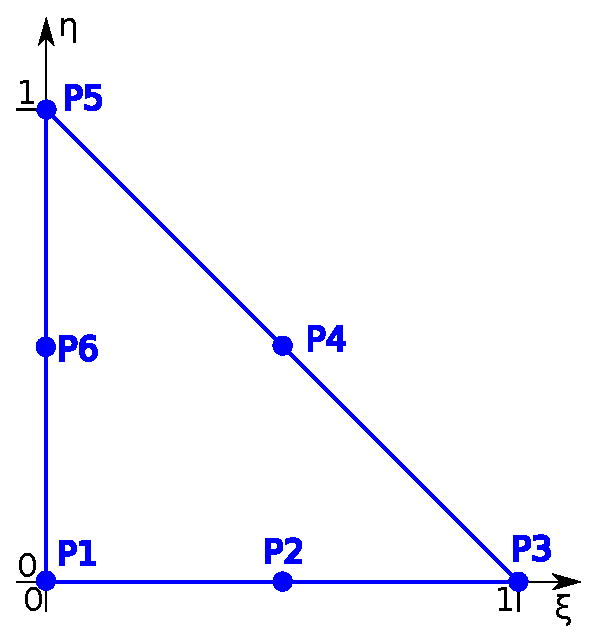
\includegraphics[scale=0.65]{pics/quadratic_element.eps}
	\end{center}
	\caption{Ansatz für quadratisches Element}
	\label{fig:quadratic_element}
\end{wrapfigure}

Der Ansatz der Potentialfunktion wird wie folgt gewählt:
\begin{equation}
\label{eq:quadratic_triangle_eq}
u(\xi, \eta) = c_0 + c_1 \xi + c_2 \eta + c_3 \xi \eta + c_4 \xi^2 + c_5 \eta^2
\end{equation}	
Nach dem Einsetzen der Knotenkoordinaten ergeben sich folgende Gleichungen zur Bestimmung der Unbekannten $c_j$:
\begin{align}
&u(0,0) = u_1 = c_0\\
&u(\nicefrac{1}{2}, 0) = u_2 = c_0 + \frac{1}{2} c_1 + \frac{1}{4} c_4 \nonumber \\
&u(1, 0) = u_3 = c_0 + c_1 + c_4 \nonumber \\
&u(\nicefrac{1}{2}, \nicefrac{1}{2}) = u_4 = c_0 + \frac{1}{2} c_1 + \frac{1}{2} c_2 + \frac{1}{4} c_3 + \frac{1}{4} c_4  \nonumber \\ 
&\quad \quad \quad \quad \quad \quad \quad \quad \ +\frac{1}{4} c_5\nonumber \\
&u(0, 1) = u_5 = c_0 + c_2 + c_5 \nonumber \\
&u(\nicefrac{1}{2}, 0) = u_6 = c_0 + \frac{1}{2} c_2 + \frac{1}{4} c_5 \nonumber
\end{align}		

Durch Anwendung des gleichen Prinzips wie in Abschnitt \ref{sec:linear_triangles} können nun die Formfunktionen $N_1 \text{...} N_6$ ermittelt werden. Diese finden sich in Anhang ... .




% =============================== Kubische Elemente ======================================

\subsubsection{Kubische Dreieckselemente}

Das kubische isoparametrische finite Dreieckselement ist wie in Abbildung \ref{fig:cubic_element} definiert.

\begin{wrapfigure}{r}{8cm}
	\vspace{-6cm}
	\begin{center}
		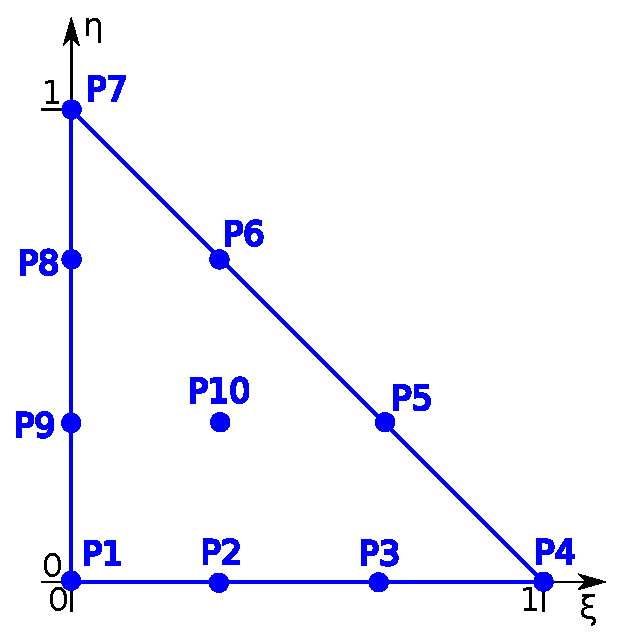
\includegraphics[scale=0.65]{pics/cubic_element.eps}
	\end{center}
	\caption{Ansatz für quadratisches Element}
	\label{fig:cubic_element}
\end{wrapfigure}

Die Koordinaten der drei Elementknoten lauten wie folgt:
\begin{align}
&P_1 = \coord{0}{0}, \quad P_2 = \coord{\nicefrac{1}{3}}{0}\\
&P_3 = \coord{\nicefrac{2}{3}}{0}, \quad P_4 = \coord{1}{0} \nonumber \\
&P_5 = \coord{\nicefrac{2}{3}}{\nicefrac{1}{3}}, \quad P_6 = \coord{\nicefrac{1}{3}}{\nicefrac{2}{3}} \nonumber\\
&P_7 = \coord{0}{1}, \quad P_8 = \coord{0}{\nicefrac{2}{3}} \nonumber \\
&P_9 = \coord{0}{\nicefrac{1}{3}}, \quad P_10 = \coord{\nicefrac{1}{3}}{\nicefrac{1}{3}} \nonumber\\
\end{align}

Der Ansatz der Potentialfunktion wird wie folgt gewählt:

\begin{equation}
\label{eq:cubic_triangle_eq}
u(\xi, \eta) = c_0 + c_1 \xi + c_2 \eta + c_3 \xi \eta + c_4 \xi^2 + c_5 \eta^2 + c_6 \xi^2 \eta + c_7 \xi \eta^2 + c_8 \xi^3 + c_9 \eta^3
\end{equation}	



Nach dem Einsetzen der Knotenkoordinaten ergeben sich folgende Gleichungen zur Bestimmung der Unbekannten $c_j$:
\begin{align}
u(0,0) = &u_1 = c_0\\
u(\nicefrac{1}{3}, 0) = &u_2 = c_0 + \frac{1}{3} c_1 + \frac{1}{9} c_4 +  \frac{1}{27} c_8\nonumber \\
u(\nicefrac{2}{3}, 0) = &u_3 = c_0 + \frac{2}{3} c_1 + \frac{4}{9} c_4 +  \frac{8}{27} c_8\nonumber \\
u(1,0) = &u_4 = c_0 + c_1 + c_4 + c_8\nonumber\\
u(\nicefrac{2}{3}, \nicefrac{1}{3}) = &u_5 = c_0 + \frac{2}{3} c_1 +  \frac{1}{3} c_2 + \frac{2}{9} c_3 +  \frac{4}{9} c_4 + \frac{1}{9} c_5 + \frac{4}{27} c_6 + \frac{2}{27} c_7 + \frac{8}{27} c_8 + \frac{1}{27} c_9\nonumber\\
u(\nicefrac{1}{2}, 0) = &u_6 = c_0 + \frac{1}{3} c_1 +  \frac{2}{3} c_2 + \frac{2}{9} c_3 +  \frac{1}{9} c_4 + \frac{4}{9} c_5 + \frac{2}{27} c_6 + \frac{4}{27} c_7 + \frac{1}{27} c_8 + \frac{8}{27} c_9\nonumber\\
u(0,1) = &u_7 = c_0 + c_2 + c_5 + c_9\nonumber\\
u(0, \nicefrac{2}{3}) = &u_8 = c_0 + \frac{2}{3} c_2 + \frac{4}{9} c_5 +  \frac{8}{27} c_9\nonumber \\
u(0, \nicefrac{1}{3}) = &u_9 = c_0 + \frac{1}{3} c_2 + \frac{1}{9} c_5 +  \frac{1}{27} c_9\nonumber \\
u(\nicefrac{1}{3}, \nicefrac{1}{3}) = &u_{10} = c_0 + \frac{1}{3} c_1 +  \frac{1}{3} c_2 + \frac{1}{9} c_3 +  \frac{1}{9} c_4 + \frac{1}{9} c_5 + \frac{1}{27} c_6 + \frac{1}{27} c_7 + \frac{1}{27} c_8 + \frac{1}{27} c_9\nonumber
\end{align}	
	

Durch Anwendung des gleichen Prinzips wie in Abschnitt \ref{sec:linear_triangles} können nun die Formfunktionen $N_1 \text{...} N_10$ ermittelt werden. Diese finden sich in Anhang ... .